\chapter{Ensemble Methods}\label{ch:ensemble-methods}

\index{Ensemble methods|(}

An ensemble is a method used in machine learning to combine predictions made by multiple learning algorithms to achieve better predictive performance \citep{clemen1989combining, perrone1993improving}. This technique works with classification problems, for example predicting whether a company will go bankrupt \citep{zikeba2016ensemble}, and it also works with regression problems, for example predicting crude oil prices \citep{yu2008forecasting}. The simplest ensemble technique used in classification problems is to take the maximum vote of all outputs made by each classifier. On the other hand, averaging the predictions made by each predictor is the most basic technique used for regression problems.   

The general idea behind ensembles is to merge each learner's hypothesis into one with the intention of obtaining better predictions. There are various ensemble methods, some of which use a single base learner to produce homogeneous learners while others use individual learners to produce heterogeneous learners. Generally, ensemble methods are applied to supervised learning algorithms. The methods described below are the most common used ensemble techniques in machine learning.

\section{Bagging}
\index{Ensemble methods!bagging|(}
\textit{Bagging}\index{Ensemble methods!bagging}, also referred to as \textit{Bootstrap Aggregating}\index{Ensemble methods!bagging!bootstrap aggregating}, is a technique introduced by \citet{breiman1996bagging}. In his work it was shown that classification and regression trees \citep{breiman1993classification} can have a significant increase in accuracy when combined with \textit{Bagging}\index{Ensemble methods!bagging}. 

This method works by sampling the training dataset into multiple subsets or bags of equal parts. These subsets are sampled using replacement, meaning that an instance can be found in multiple subsets. The size of each subset is defined as a percentage of the total size of the training dataset. Once the training set is sampled, each subset is utilized to fit a different learner. A prediction $\hat{y}$ on an unforeseen instance $x$ is made by taking a maximum vote made by each learner as the predicted classification as shown in Equation~\ref{eq:baggingvote}. If it is a regression problem an average of the predicted values is taken as the final output as shown in Equation~\ref{eq:baggingmean}. This procedure can be better visualized in Figure~\ref{fig:baggingexample}. The idea behind this technique is to avoid overfitting by reducing variance.

\begin{equation}\label{eq:baggingvote}
    f(x) = argmax \sum_{b=1}^{B} f_b(y | x)
\end{equation}

\begin{equation}\label{eq:baggingmean}
    f(x) = \frac{1}{B} \sum_{b=1}^{B} f_b(x)
\end{equation}

\begin{figure}
  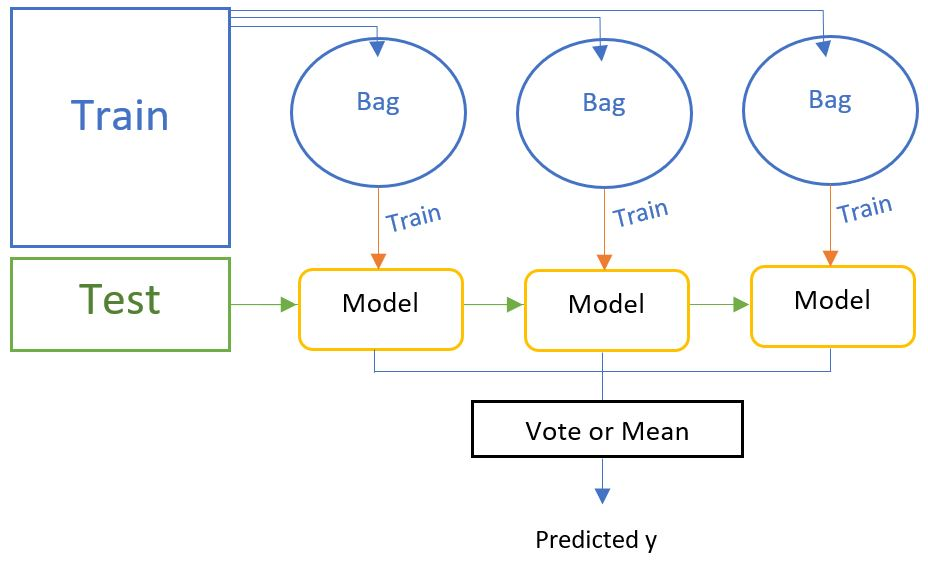
\includegraphics{graphics/ensemble_methods/bagging_example.JPG}
  \caption{
    Dataset Bagging using 3 base learners. Each bag is a subset of the training set. Instances are selected randomly and with replacement. Each base learner is fitted with the respective bag. Predictions are then made by each base learner and the final output $\hat{y}$ is the maximum vote or an averaged value of all predictions. 
  }
  \label{fig:baggingexample}
\end{figure}

\textit{Bagging} can also be applied to the feature set where subsets of the features is selected at random and used to fit the base learners. This technique is referred to as \textit{Feature Bagging}\index{Ensemble methods!bagging!feature bagging}. One popular model that utilizes \textit{Feature Bagging} is \textit{Random Forests}\index{Ensemble methods!bagging!random forests} introduced by \citet{ho1995random}. It uses multiple \textit{Decision Trees}\index{Ensemble methods!bagging!decision trees} which are trained using subsets of the total feature set selected at random. It was shown that when applying this method with multiple \textit{Decision Trees}, the model was able to generalize more when classifying handwritten digits. An extension to \textit{Random Forests} was later developed which uses both \textit{Bagging} and \textit{Feature Bagging} to further control variance \citep{breiman2001random}.

\index{Ensemble methods!bagging|)}

\section{Boosting}
\index{Ensemble methods!boosting|(}
This technique is a variation on \textit{Bagging} which aims to improve the learner's predictive performance by correcting the errors made by the previous learners in the ensemble, hence the name \textit{Boosting}. The idea of having multiple \textit{weak learners}\index{Ensemble methods!boosting!weak learners} that adapt by correcting errors was introduced by \citet{freund1997decision} and this technique is called \textit{Adaptive Boosting}\index{Ensemble methods!boosting!adaptive boosting} or \textit{AdaBoost}, which is the most common \textit{Boosting} method. It was shown that this technique can reduce both bias and variance \citep{breiman1996bias}. \textit{AdaBoost} does not work well when having insufficient data or very weak hypotheses \citep{freund1999short}. It also suffers when having a large number of outliers in the dataset and can significantly reduce the predictive performance \citep{dietterich1998experimental}. Variants of \textit{AdaBoost} were developed to combat large amount of outliers in the dataset such as \textit{'Gentle AdaBoost'}\index{Ensemble methods!boosting!gentle adaboost} which gives less importance to outliers \citep{friedman2000additive} and \textit{'BrownBoost'}\index{Ensemble methods!boosting!brown boost} which uses a combination of Brownain motion, \textit{Boosting} and repeated games to handle such cases \citep{freund2001adaptive}.  

\textit{Boosting} works by taking a subset of the training set to train the first learner. Once the learner is trained, it is validated using the whole training set. When validation is done, each instance in the original dataset is given a weight based on the error made by this learner. A new learner is now trained on a new subset, but this time instances with higher weights are more likely to be selected. Again, this learner is validated using the whole training set but the weights for each instance is now recalibrated using a combined prediction of the two learners as shown in Figure~\ref{fig:boostingexample}. This process goes on for the number of learners specified to be used in the ensemble and the idea behind it is that each learner corrects the previous learner's errors.  Once this procedure is finished, a prediction is made on the weighted mean of each learner if it is a regression problem as shown in Equation~\ref{eq:boostinggmean}. If it is a classification problem, it takes a weighted vote to come up with the predicted classification  as shown in Equation~\ref{eq:boostingvote}. 

\begin{figure}
  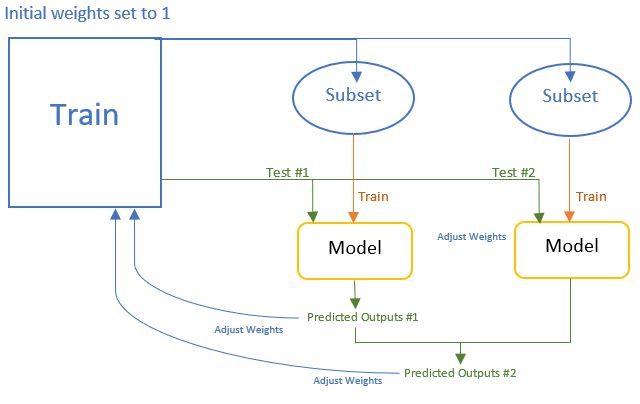
\includegraphics{graphics/ensemble_methods/boosting_example.JPG}
  \caption{
     Boosting using 2 base learners. Initially weights are set to 1, so all instances have the same probability to be selected in the subset. The first learner is trained using the first subset and then validated using the whole training set. Weights are recalibrated depending on the errors of the predictions. On the second run, instances which had significant errors are more likely to be selected. The second learner is now trained and tested using the whole training set. This time weight are adjusted using the combined predictions of the two learners.  
  }
  \label{fig:boostingexample}
\end{figure}

\begin{equation}\label{eq:boostinggmean}
    f(x) = \frac{1}{B} \sum_{b=1}^{B} \alpha_b f_b(x)
\end{equation}

\begin{equation}\label{eq:boostingvote}
    f(x) = sign (\sum_{b=1}^{B} \alpha_b f_b(y | x))
\end{equation}

This technique assumes that the learners are 'weak' and homogeneous. \textit{Boosting} aims to build a stronger learner by combining a collection of \textit{weak learners}\index{Ensemble methods!boosting!weak learners}. \textit{Boosting} works in sequence and cannot be parallelized since the learners are dependent on each other. There are various other variations of boosting but one other popular implementation worth mentioning is \textit{Gradient Boosting}\index{Ensemble methods!boosting!gradient boosting} 'GBM' which focuses on optimizing the loss function using boosting \citep{breiman1997arcing}. 
\index{Ensemble methods!boosting|)}

\section{Stacking}
\index{Ensemble methods!stacking|(}
\textit{Stacking} or \textit{Stacked Generalization}\index{Ensemble methods!stacking!stacked generalization} is an ensemble method introduced by \citet{wolpert1992stacked}, it aims to reduce the generalization error of the combined model. Unlike the previous techniques it can be used to combine heterogeneous learners. In fact, this technique works better when the learners are different from each other and are known to be strong learners.  

In \textit{Stacking}, the dataset is first split into two; the training set and the test set. The training set is further split into K-folds like the K-fold cross validation technique. Each learner is then trained on $K-1$ folds and validation is done on the holdout fold. For prediction made by each learner at the holdout fold is recorded and stacked together to form a new dataset. The actual value/label is also stacked at the end. This procedure continues for $K$ times. Once all the learners have been trained using this method, a new dataset would be created with the predictions made by each learner which will be used as features. This dataset is then used to train the \textit{combiner learner}\index{Ensemble methods!stacking!combiner learner}, which is also referred to as the \textit{meta-model}\index{Ensemble methods!stacking!meta-model} or the \textit{aggregator model}\index{Ensemble methods!stacking!aggregator model} as shown in Figure~\ref{fig:stackingexample}. After this model is trained using this newly generated dataset it will be validated using the original test set. 

When using \textit{Stacking} for classification it is advised to use class probabilities instead of the predicted outcomes as it gives a better measure of confidence for each model, thus enhancing the meta-dataset \citep{ting1999issues}. 

\begin{figure}
  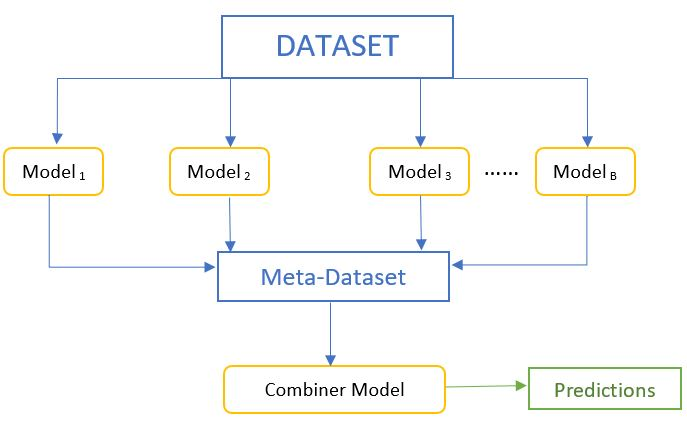
\includegraphics{graphics/ensemble_methods/stacking_example.JPG}
  \caption{
     A visual representation of the steps required when Stacking multiple machine learning models.
  }
  \label{fig:stackingexample}
\end{figure}

The general idea behind this ensemble technique is to combine multiple different learners together, but unlike the previous methods, \textit{Stacking} combines the models using another intermediate model which is trained on the predictions made by individual learners. \textit{Stacking} technique was also studied to identify Higgs bosons at the Large Hadron Collider where \textit{Stacking} outperformed \textit{Boosted Decision Trees}\index{Ensemble methods!stacking!boosted decision trees} \citep{alves2017stacking}.  
\index{Ensemble methods!stacking|)}

\index{Ensemble methods|)}